%\documentclass{exam} 
\documentclass[answers]{exam} 
\usepackage{amsmath,amssymb,enumitem,fdsymbol,float,tikz,etoolbox,ifthen,xcolor,fullpage,ulem,graphicx, comment,hyperref} 
\usepackage{tikz}
\usepackage{pgfplots}
\pgfplotsset{compat=1.11}
\usepgfplotslibrary{fillbetween}
\usetikzlibrary{intersections}

\pgfdeclarelayer{bg}
\pgfsetlayers{bg,main}
\usetikzlibrary {arrows.meta,calc}
\addpoints
\marksnotpoints

\AtBeginEnvironment{solution}{\color{red}}

%Add rubrics
%\usepackage{tagging}
\usepackage[rubric]{tagging}

%\newcommand\rubric[1]{\tagged{rubric}{\color{blue}{#1}\color{black}}}
\newcommand\rubric[1]{\tagged{rubric}{\color{blue}}}

\setlength\parindent{0in}
%\pagestyle{empty}

\everymath{\displaystyle}
\newcommand{\dee}{\,\text{d}}
\newcommand{\diff}[2]{\frac{\text{d}#1}{\text{d}#2}}

\begin{document}

\large{\textbf{Optimization and the carbon tax, Math 100}}

Peter Harrington

\normalsize
\hrulefill

\

In this assignment we will examine the effect a carbon tax has on the production of oil. Economists often use marginal revenue and marginal cost curves to understand the quantity of a resource a company will extract. Say there is an oil company with an oil well. As the company drills more oil, the remaining oil is harder to access, so the more oil the company produces, the more expensive it becomes to extract an additional unit of oil. This can be quantified in terms of marginal cost, which is the cost of extracting one more unit of oil. In this scenario the marginal cost to extract some additional quantity, $q$ of oil is: \[\text{Marginal Cost}: MC(q)= c+dq,\] where the units of marginal cost are dollars/unit and $c$ and $d$ are positive constants. The total cost to the company of producing $q$ units of oil can then be found by taking the area under the marginal cost curve. Intuitively the area under the marginal cost curve represents the sum of the marginal costs for each unit of oil produced, which would be the total cost of producing $q$ units. The idea of area as a sum is explored in much more detail in Math 101.

\

At the same time, consumers are willing to pay more when there is less oil, and are less willing to pay as much when there is more oil. If we assume the oil company has a monopoly on oil extraction then the marginal revenue that the company can make on some additional quantity, $q$, of oil is: \[\text{Marginal Revenue}: MR(q)=a-bq,\] where the units of marginal revenue are dollars/unit and $a$ and $b$ are positive constants. The total revenue a company gains by producing $q$ units of oil can then be found by taking the area under the marginal revenue curve. 


\

The total profit that a company makes by producing $q$ units of oil can be found by subtracting the area under the marginal cost curve (total cost) from the area under the marginal revenue curve (total revenue).

\

\begin{questions}
    

 
\question ($\bigstar \bigstar \bigstar \largewhitestar$) 

\begin{parts}
    \part Find the area as a function of $q$, $A_c(q)$, below the marginal cost curve, $MC(q)=c+dq$, where $c>0$ and $d>0$. $A_c(q)$ is the shaded area shown in the figure below. The area under the marginal cost curve, $A_c(q)$, represents the total cost to the company to produce $q$ units of oil.
    
    
    Hint: divide the area under the curve $MC(q)$ into the area of a triangle and the area of a rectangle and add them together. The width of the rectangle is $q$ and the height of the rectangle is $c$.
    
        \begin{center}
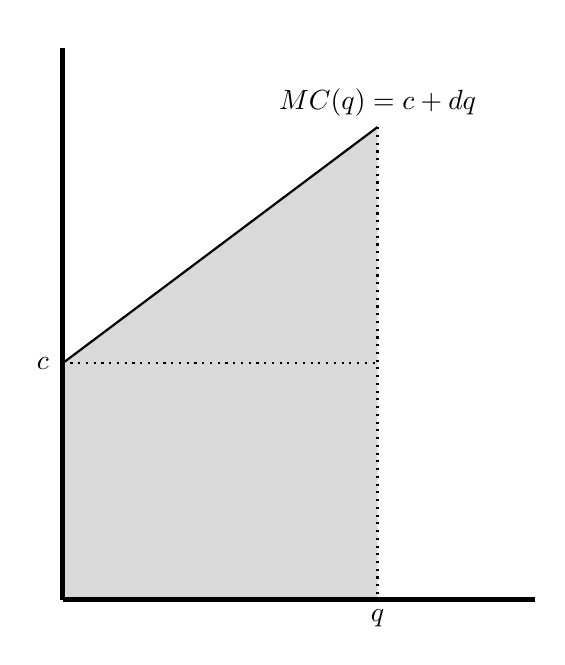
\begin{tikzpicture}[thick,yscale=1]
\draw[fill=gray!30, draw=none ] (0,0) -- (4,0) -- (4,6) -- (0,3);
\draw[ultra thick, name path =D ] (6,0) -- (0,0) node[left]{};
%\node[circle,fill=black,inner sep=0pt,minimum size=5pt,label=left:{you}] (a) at (0,0) {};
%\node[] at (3,0.5) {ground};
%\node[] at (3,-1) {10m};
\draw[ultra thick, name path=A] (0,0) -- (0,7) node[above]{};
%\node[] at (6.5,2) {tree};
\draw[name path=B] (0,3) -- (4,6) node[above]{$MC(q)=c+dq$};
\draw[dotted] (0,3) -- (4,3) node[]{};
\node[] at (-0.25,3) {$c$};
\draw[dotted, name path =C] (4,6) -- (4,0) node[below]{$q$};
%\draw[->] (5,3.1) -- (3,4);
%\draw[->] (5,2.9) -- (3,2);
%\node[] at (5.5,3) {$A_c(q)$};
%\node[] at (.75,.25) {$\theta$};
%\node[] at (5.6,6) {cat};
%\node[rotate=45] at (3, 3.75) {leash};
%\node[] at (6,7.25) {squirrel};
\end{tikzpicture}
\end{center}

\part Find the area as a function of $q$, $A_r(q)$, below the marginal revenue curve, $MR(q)=a-bq$, for $q\in [0,\frac{a}{b}]$. Here $a>0$ and $b>0$. The area under the marginal revenue curve, $A_r(q)$, represents the total revenue the company gains by producing $q$ units of oil.

Hint: again divide the area under the curve $MR(q)$ into the area of a triangle and the area of a rectangle and add them together. The width of the rectangle is $q$ and the height is $a-bq$.

        \begin{center}
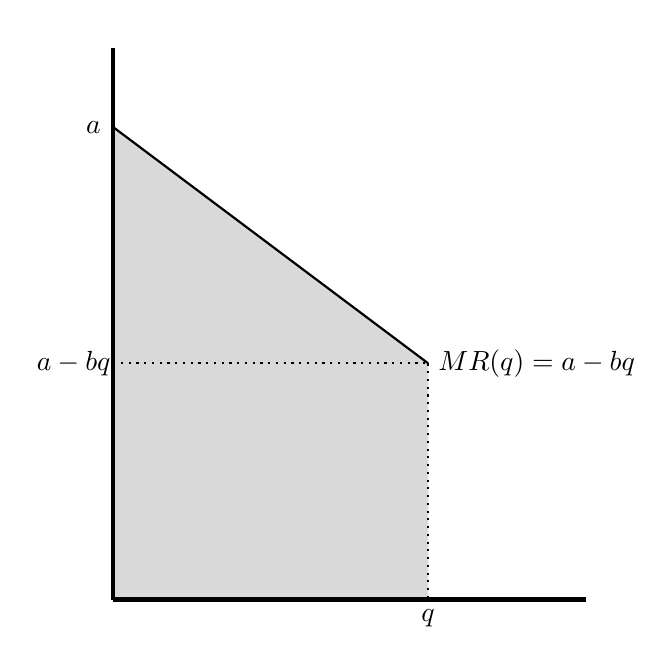
\begin{tikzpicture}[thick,yscale=1]
\draw[fill=gray!30, draw=none ] (0,0) -- (4,0) -- (4,3) -- (0,6);
\draw[ultra thick, name path =D ] (6,0) -- (0,0) node[left]{};
%\node[circle,fill=black,inner sep=0pt,minimum size=5pt,label=left:{you}] (a) at (0,0) {};
%\node[] at (3,0.5) {ground};
%\node[] at (3,-1) {10m};
\draw[ultra thick, name path=A] (0,0) -- (0,7) node[above]{};
%\node[] at (6.5,2) {tree};
\draw[name path=B] (0,6) -- (4,3) node[right]{$MR(q)=a-bq$};
\draw[dotted] (0,3) -- (4,3) node[]{};
\node[] at (-0.5,3) {$a-bq$};
\node[] at (-0.25,6) {$a$};
\draw[dotted, name path =C] (4,3) -- (4,0) node[below]{$q$};
%\draw[->] (5,3.1) -- (3,4);
%\draw[->] (5,2.9) -- (3,2);
%\node[] at (5.5,3) {$A_c(q)$};
%\node[] at (.75,.25) {$\theta$};
%\node[] at (5.6,6) {cat};
%\node[rotate=45] at (3, 3.75) {leash};
%\node[] at (6,7.25) {squirrel};
\end{tikzpicture}
\end{center}
    
    
    \part Assume that $a>c$ and $q\in [0,\frac{a}{b}]$. The total profit the oil company makes as a function of quantity produced, $q$, is given by $P(q)=A_r(q)-A_c(q)$. Find the quantity $q^*$ that the company should produce in order the maximize its profit. Make sure to justify why the quantity you found is indeed the global maximum.

    \part What is the total profit that the company makes when it is producing the quantity which maximizes its profit? In other words, what is $P(q^*)$?

    \part Another method of finding the quantity $q^*$ that the company should produce in order the maximize its profit is to look for where $MR(q)$ and $MC(q)$ intersect. Why should this intersection point be where profit is maximized?



\end{parts}
\end{questions}


 In the scenario above, the oil company will typically produce the quantity of oil that maximizes its profit, with no consideration to the climate emissions produced in the extraction of oil. One method that governments use to reduce the climate emissions involved in the extraction of oil is to impose a carbon tax on the fuel used to extract oil. In BC, the carbon tax is currently \$65/tonne. This essentially increases the marginal cost of producing some quantity $q$ of oil by some fixed positive amount $t$.

\begin{questions}\setcounter{question}{2}
\question ($\bigstar \bigstar \bigstar \largewhitestar$) 
Assume the carbon tax is applied so that the Marginal Cost is now $MC_t(q)=c+t+dq$ and that $a>(c+t)$. 
\begin{parts}
\part What is the quantity produced by the oil company that maximizes profits now? For the other parts of this question, call this quantity $\Tilde{q}$. The profit function is now $P_1(q)=A_r(q)-A_{ct}(q)$, where $A_{ct}(q)$ is the area under the new marginal cost curve, $MC_t(q)$. Assume again that $q\in[0,\frac{a}{b}]$ and make sure to justify why the quantity you found is indeed the global maximum.

    \part  What is the total profit that the company makes when it is producing the quantity which maximizes its profit now? In other words, what is $P_1(\Tilde{q})$?

    \part Is the new quantity where profit is maximized, $\Tilde{q}$, less than the quantity that maximized profit with no carbon tax, $q^*$?
    \part How big does the carbon tax, $t$, need to be so that the new quantity produced where profit is maximized is half of the old quantity produced? In other words, how big does $t$ need to be in order for $\Tilde{q}=\frac{q^*}{2}$? 
\end{parts}

\begin{comment}
\question  ($\bigstar \bigstar \bigstar \largewhitestar$) 

 Sometimes a fixed marginal revenue function can be a better descriptor of revenue than the decreasing marginal revenue function used in the first part of the assignment. Let the fixed marginal revenue be \[\text{Marginal Revenue}:MR(q)=c+d\left( \frac{a-c}{b+d}\right),\] so that if there is no carbon tax, the quantity that maximizes profit is the same as found in the first part of this assignment. Using this new function for marginal revenue, find the optimal quantity, $q$, the oil company should produce to maximize total profit if the carbon tax is introduced, where $\text{Marginal Cost}=c+t+dq$. Is this quantity larger or smaller than the one found in Q6?
\end{comment}





\end{questions}

\end{document}
